We use finite-size DMRG \cite{catarina_density-matrix_2023, Fishman_2022}, with the primary results presented for a lattice with $L=30$ sites, a cutoff $\sub{n}{c} = 5$, open boundary conditions, and a bond dimension $D=300$ (unless otherwise specified). Fixing $U=1$, we examine the system's behavior in the $(t, \mu)$-plane\textsuperscript{\footnote{
     The parameter $t$ represents the hopping amplitude between neighboring sites, $U$ denotes the on-site interaction strength, and $\mu$ is the chemical potential controlling the particle number.
}}.


\begin{figure}[t]
    \centering
    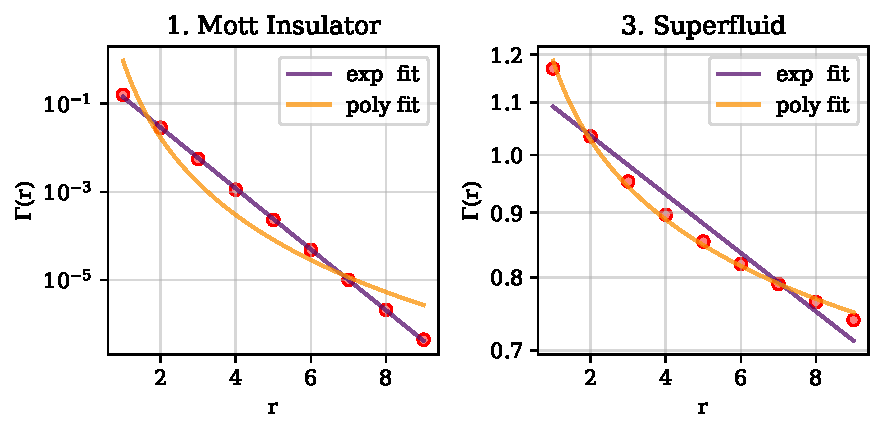
\includegraphics[width=\linewidth]{imgs/decay.pdf}
    \caption{Demonstration of the exponential decay of $\Gamma(r)$ for MI (1) and polynomial decay for SF (3).}
    \label{fig:decay}
\end{figure}


\begin{figure}[b]
    \centering
    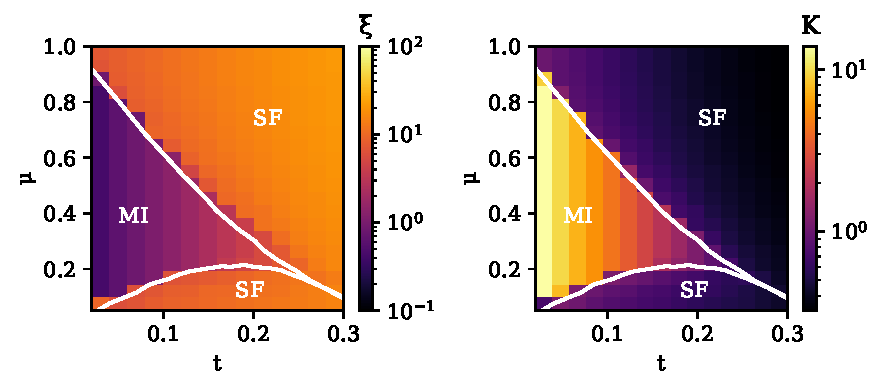
\includegraphics[width=\linewidth]{imgs/phases2.pdf}
    \caption{Phases of the 1D Bose-Hubbard model. Phase boundaries are drawn according to the results from \cite{kuehner_phases_1998}. Near the boundaries, the divergence of $\xi$ and the approach of $K$ to the critical value $\sub{K}{c}=1/2$ can be observed.}
    \label{fig:phases2}
\end{figure}





\begin{figure*}
    \centering
    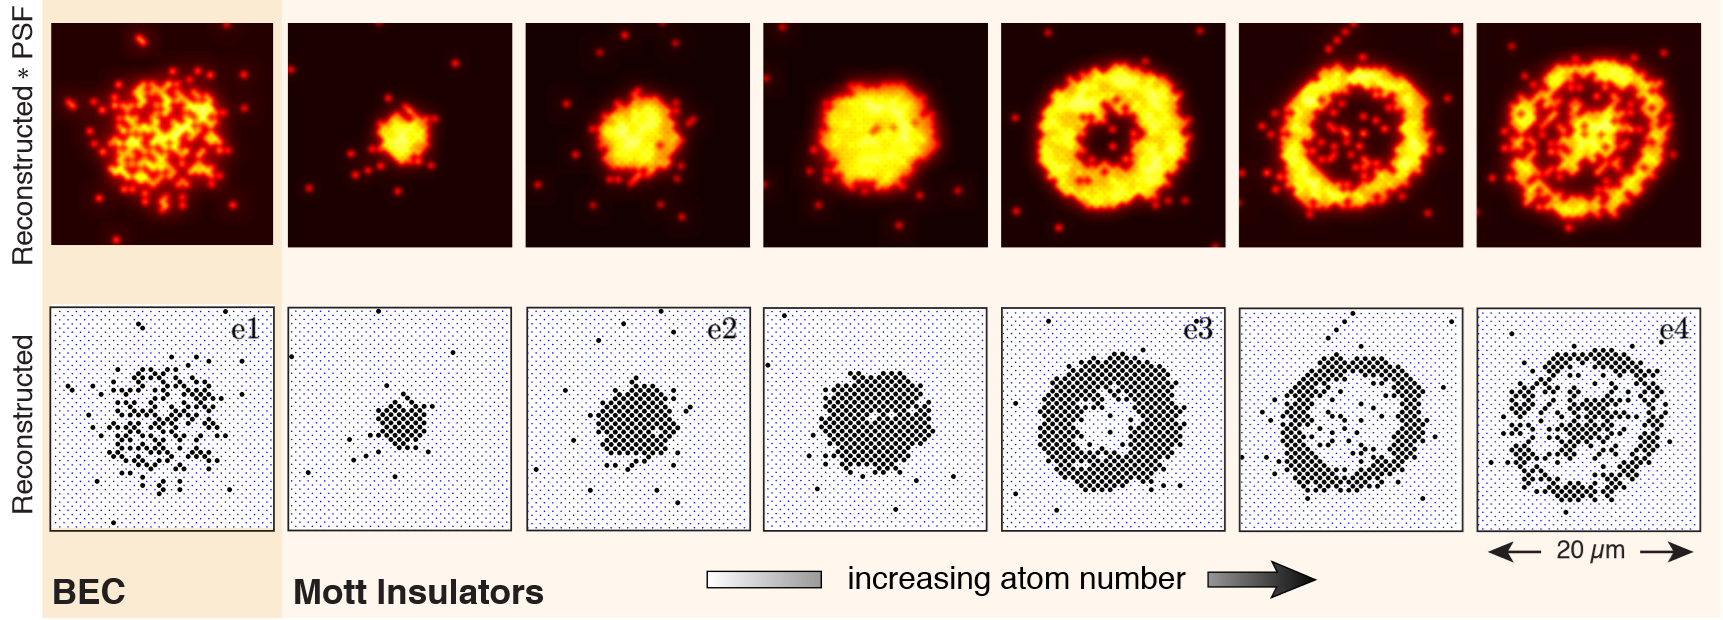
\includegraphics[width=\textwidth]{imgs/MIexp.png}
    \caption{High-resolution fluorescence images of a BEC (SF) and Mott insulators (MI) with in-plane harmonic confinement from \cite{sherson_single-atom-resolved_2010}. Experimentally obtained images of a BEC (e1) and Mott insulators for increasing particle numbers (e2, e3, e4) in the zero-tunneling limit, showing $\langle n_j \rangle \mod 2$. Clear integer filling of the lattice with $n=1, 2, 3$ can be observed.}
    \label{fig:MIexp}
\end{figure*}



Through $\xi$ and $K$, we can obtain information about particle mobility and correlations. A  correlation length larger $\xi$ signifies longer-range correlations, indicating the extent of coherence in the system, typical in the superfluid phase, while a smaller $\xi$ indicates short-range correlations, characteristic of the Mott insulator phase. 

The correlation length can be determined in two ways: first, by definition,
\begin{equation*}
	\xi(r) = \frac{\sum_r r^2 \Gamma(r)}{\sum_r \Gamma(r)},
\end{equation*}
although this approach is more sensitive to the finite size of the system. Alternatively, assuming an exponential decay $\sub{\Gamma}{MI}(r) \propto e^{-r/\xi}$, $\xi$ can be found through fitting the calculated correlator, which works well in the MI region. Similarly, by fitting the decay in the SF and critical regions, where we expect a polynomial decay, we can determine the exponent $K$ via $\sub{\Gamma}{SF}^2(r) \propto r^{-K}$. The results of fitting\textsuperscript{\footnote{
  One could assume that the function $e^{-r/\xi} / r^{K/2}$ would describe the decay well across the entire phase space. However, such a fit is more unstable, and the phases can still be distinguished throughout the space by either $K$ or $\xi$.
}} with these two functions are presented in Fig. \ref{fig:decay}, where it is evident that the decay is exponential for MI and polynomial for SF
% \textsuperscript{\footnote{
% 	One could assume that the function $e^{-r/\xi} / r^{K/2}$ would describe the decay well across the entire phase space. However, such a fit is more unstable, and the phases can still be distinguished throughout the space by either $K$ or $\xi$.
% }}.

Additionally, the average number of particles per site $\langle n_j \rangle$ is a crucial indicator of the MI phase. In the MI phase, $\langle n_j \rangle$ is typically an integer (fig. \ref{fig:MIexp}), reflecting the fixed number of particles due to strong repulsive interactions, when particle mobility is suppressed, and the system is incompressible. In contrast, in the superfluid phase, $\langle n_j \rangle$ can vary continuously, indicating higher particle mobility and the absence of a gap for particle-hole excitations. To quantify the deviation from integer filling, we introduce $\delta n_j = n_j - 1$, which helps in analyzing the fluctuations and transitions between the phases.




\section{Phase Diagram}

For $t \in[0, 0.3]$ in steps of $0.02$ and $\mu \in [0, 1]$ in steps of $0.05$ at $U=1$, the correlators $\Gamma_{ij}$ were calculated. From these, the values of $\xi$ and $K$ were obtained through fitting, and the results are presented in Fig. \ref{fig:phases2}. The correlation length exhibits a sharp divergence near the critical point $\ln \xi \sim 1 / \sqrt{t_c - t}$ 
subject to finite size limitations. The critical exponent $\sub{K}{c}$ of the phase transition is also known from Luttinger liquid theory \cite{PhysRevB.46.9325,kuehner_phases_1998}. At the BKT transition with $\langle n_j \rangle = 1$, $K$ is expected to be $\sub{K}{c} = 1/2$. However, even without this knowledge, it is quite possible to distinguish the two regions based on $K$. In this context, Luttinger liquid theory simply helps to define this boundary more precisely. The divergence of $\xi$ and the critical value $K = \sub{K}{c}$ are in complete agreement with the phase boundaries defined in \cite{kuehner_phases_1998}.


\begin{figure}[b]
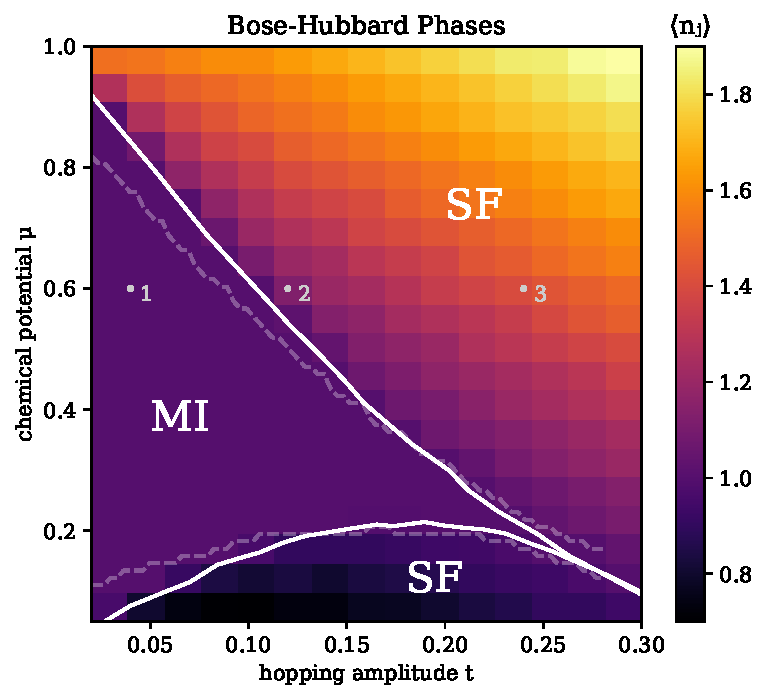
\includegraphics[width=0.9\linewidth]{imgs/phases.pdf}
\caption{The average number of particles per site. It is evident that the filling is strictly one in the MI region.}
\label{fig:phases}
\end{figure}


\begin{figure*}[t]
    \centering
    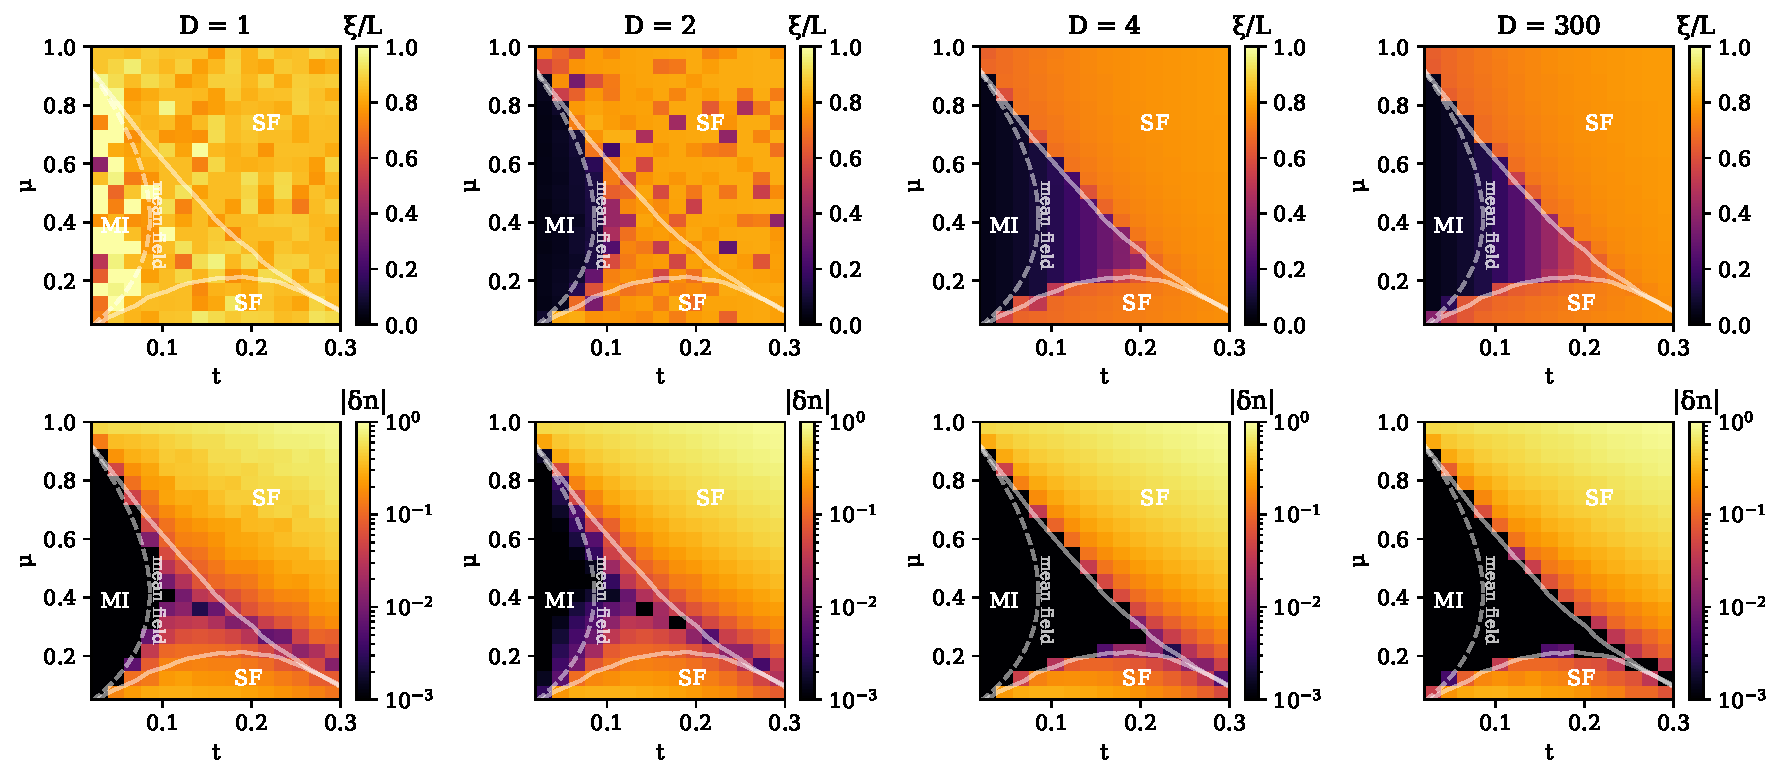
\includegraphics[width=\textwidth]{imgs/phases2mf.pdf}
    \caption{Phase diagrams obtained via DMRG for various bond dimensions $D$. As $D$ decreases, the solution approaches the mean field solution, both in terms of system filling and correlation length.}
    \label{fig:mf}
\end{figure*}


Note that the diagonal part of the calculated correlators $\Gamma_{jj} = n_j$, and by plotting $\langle n_j\rangle$ in the $(t, \mu)$-plane, we can clearly observe the unit filling in the MI phase (Fig. \ref{fig:phases}). The characteristic points 1, 2, and 3 used earlier for illustration are also marked here. Using linear interpolation with smoothing, we have also delineated the boundaries of the $\langle n_j\rangle = 1$ region (white dashed line), which closely align with the phase boundaries. In the SF region, increasing $\mu$ leads to a continuous and monotonic increase in the average number of particles.
